\documentclass[12pt, a4papre]{article}
\usepackage[catalan]{babel}
\usepackage[unicode]{hyperref}
\usepackage[dvipsnames]{xcolor}
\usepackage{amsmath}
\usepackage{amssymb}
\usepackage{amsthm}
\usepackage{xifthen}
\usepackage{siunitx}
\usepackage{xcolor}
\usepackage{float}
\usepackage{listings}
\usepackage{setspace}
\usepackage{graphicx}
\usepackage{tikz,lipsum,lmodern}
\usepackage[most]{tcolorbox}
\usepackage{multicol}
\usepackage{fancyvrb}
\usepackage{circuitikz}
\usepackage{indentfirst}
\usepackage{verbatimbox}
\usepackage{verbatim}
\usepackage[utf8]{inputenc}
\definecolor{mygreen}{RGB}{28,172,0} % color values Red, Green, Blue
\definecolor{mylilas}{RGB}{170,55,241}
\graphicspath{ {./Images/} }

\newcommand{\norm}[1]{\lvert #1 \rvert}

\hypersetup{
    colorlinks = true,
    linkcolor = blue
}

\author{Daniel Vilardell}
\title{Memoria practica 1 ONELE}
\date{}

\begin{document}
	\maketitle
	\textbf{Ejercicio 1:} Represente las gráficas ancho de la apertura – semiancho del haz para los casos a) y b) con Excel o con cualquier otro programa que prefiera.
	
	\textbf{a)} Siguiendo las comandas dadas en el enunciado hemos obtenido la siguiente tabla.
	\begin{center}
		\begin{tabular}{ ||c|c|| } 
			\hline
			Ancho de apertura[um]& Semiancho angular de haz[º]\\ 
			\hline
			2 & 11.28\\ 
			4 & 5.69\\ 
			6 & 3.69\\ 
			8 & 2.84\\ 
			10 & 2.27\\ 
			12 & 1.92\\ 
			14 & 1.65\\ 
			16 & 1.5\\ 
			18 & 1.29\\ 
			20 & 1.19\\ 
			\hline
		\end{tabular}
	\end{center}
	
	\begin{figure}[H]
		\begin{center}
		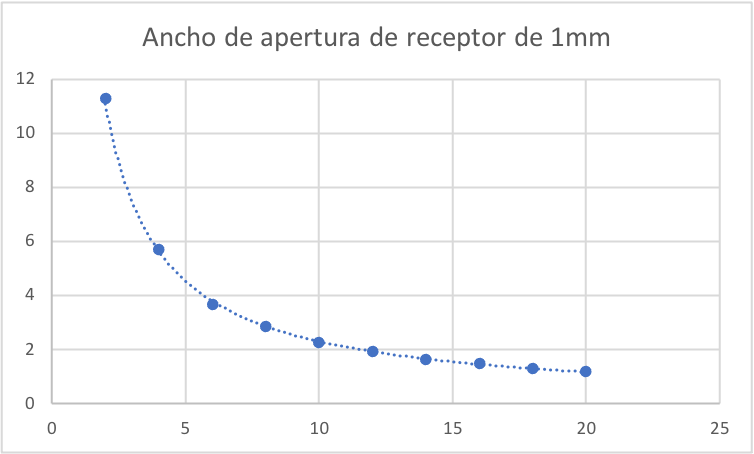
\includegraphics[width=110mm]{graph2.png}
		\caption{Semiancho angular de haz en funcion del ancho de apertura}
		\end{center}
	\end{figure}
	
	
	\textbf{b)} Con un ancho de apertura de receptor hemos obtenido la siguiente tabla.
	\begin{center}
		\begin{tabular}{ ||c|c|| } 
			\hline
			Ancho de apertura[um]& Semiancho angular de haz[º]\\ 
			\hline
			2 & 11.28\\ 
			4 & 5.9\\ 
			6 & 4.21\\ 
			8 & 3.42\\ 
			10 & 2.96\\ 
			12 & 2.7\\ 
			14 & 2.55\\ 
			16 & 2.36\\ 
			18 & 2.26\\ 
			20 & 2.16\\ 
			\hline
		\end{tabular}
	\end{center}
	
	\begin{figure}[H]
		\begin{center}
		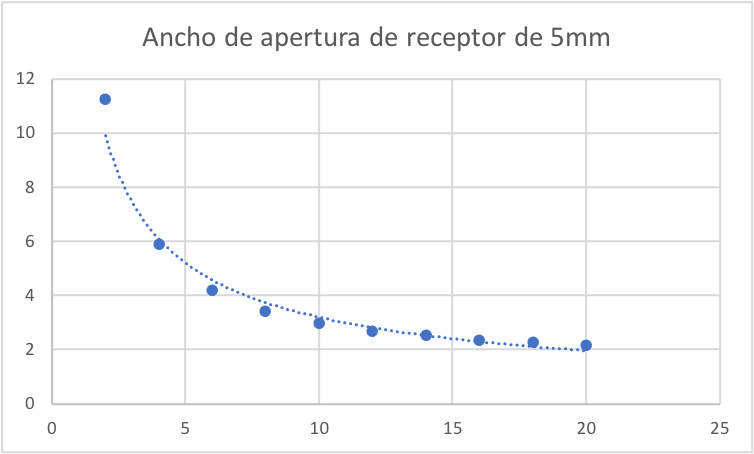
\includegraphics[width=110mm]{graph1.png}
		\caption{Semiancho angular de haz en funcion del ancho de apertura}
		\end{center}
	\end{figure}
	
	\textbf{Ejercicio 2:} En classe medimos que a una distancia de $L=30cm$ el diametro del aro principal era de $d=1.5cm$. Como sabemos que $d\ll L$ podemos usar el principio de huygens.
	
	\[
	 	\omega = \tan^{-1}\left(\frac{\frac{d}{2}}{L}\right) = \tan^{-1}\left(\frac{0.75}{30}\right) = 1.43^o
	\]
	
	Mirando entonces a la grafica observamos que $0.14mm$ corresponderia a una abertura de unas 16 micras.
	\newpage
	\textbf{Ejercicio 4:} Ajustando el simulador con los parametros dados por el enunciado llegamos a la siguiente configuración.
	
	\begin{figure}[H]
		\begin{center}
		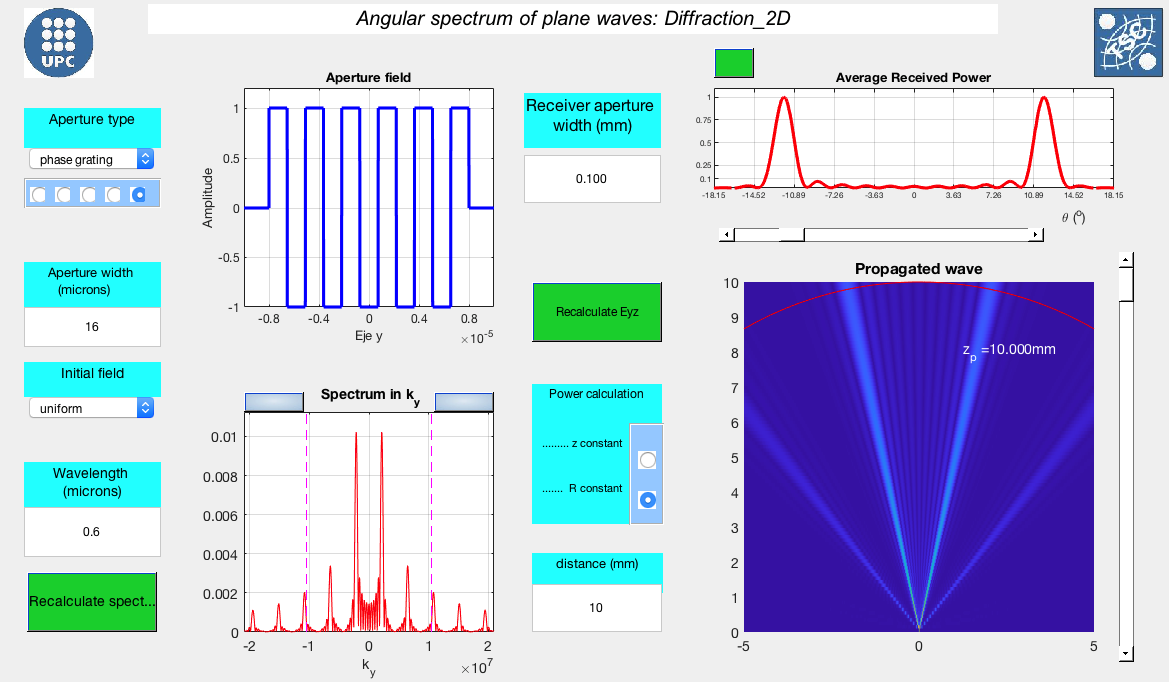
\includegraphics[width=150mm]{programa1.png}
		\caption{Configuracion ejercicio 4}
		\end{center}
	\end{figure}
	
	Medimos entonces los angulos de valores de pico en funcion del ancho de apertura y obtenemos la siguiente tabla.
	\begin{center}
		\begin{tabular}{ ||c|c|| } 
			\hline
			Ancho de apertura[um]& Semiancho angular de haz[º]\\ 
			\hline
			10 & 19.13\\ 
			12 & 15.89\\ 
			14 & 13.58\\ 
			16 & 11.86\\ 
			18 & 10.53\\ 
			20 & 9.56\\ 
			22 & 8.53\\ 
			24 & 7.89\\ 
			26 & 7.26\\ 
			\hline
		\end{tabular}
	\end{center}
	\begin{figure}[H]
		\begin{center}
		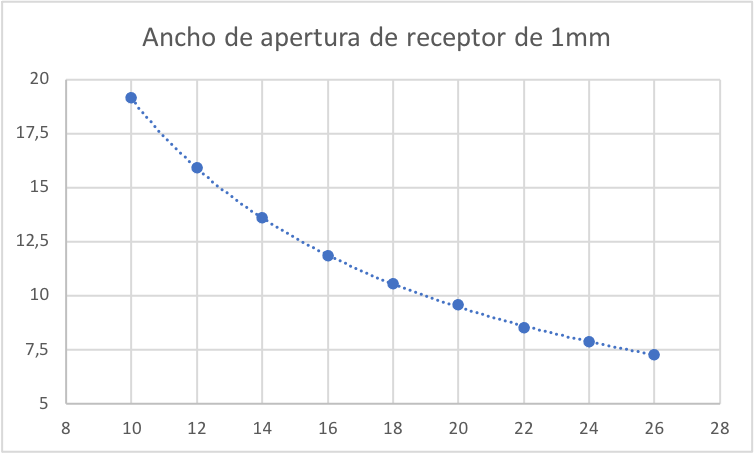
\includegraphics[width=110mm]{graph3.png}
		\caption{Semiancho angular de haz en funcion del ancho de apertura}
		\end{center}
	\end{figure}
	
	Podemos aproximar el campo en la apertura con la siguiente funcion $E(y) = E_o \cos(wy)\prod\left(\frac{y}{L}\right)$. Calculamos entonces la transformada de Fourier de la aproximación del campo en la apertura, que en angulos pequeños nos dara el campo a distancias grandes.
	
	\[
		TF\{E(y)\} = \frac{E_o}{2}Lsinc(ky\frac{L}{2}+w)+\frac{E_o}{2}Lsinc(ky\frac{L}{2}-w)
	\]
	
	De donde obtenemos que $\omega = arctg\left(\frac{\lambda \pi}{L}\right)$. Usando ahora la formula en vez de el simulador obtenemos la siguiente tabla que como podemos ver es muy similar a la encontrada a la simulación.
	\begin{center}
		\begin{tabular}{ ||c|c|| } 
			\hline
			Ancho de apertura[um]& Semiancho angular de haz[º]\\ 
			\hline
			10 & 19.20\\ 
			12 & 16.24\\ 
			14 & 13.85\\ 
			16 & 11.92\\ 
			18 & 10.63\\ 
			20 & 9.46\\ 
			22 & 8.50\\ 
			24 & 7.88\\ 
			26 & 7.20\\ 
			\hline
		\end{tabular}
	\end{center}
	
\end{document}










